%! TEX root = 'main.tex'

\section{Background}

%In this section , we talk about the background knowledge of kernel TOCTOU vulnerability, how it happens. Also SMAP feature of Intel processor, how to leverage it as the core mechanism to prevent kernel TOCTOU attacks.  

Time Of Check to Time Of Use is a class of software bug caused by changes in a system between the checking of a condition and the use of the results of that check. Normally some data changes, such as an variable. In general, it's an example of race conditions.

This issue has been addressed by many research work ~\cite{dean2004fixing}~\cite{borisov2005fixing}. A classic TOCTOU problem is something looks like this:


%\begin{lstlisting}[basicstyle=\small,style=redkeyword]
\begin{lstlisting}[basicstyle=\normalsize,style=redkeyword]
if (access(pathname, R\_OK) == 0)
    if ((fd = open(pathname, O\_RDONLY)) == 0) ...
\end{lstlisting}

This could be a piece of code in a setuid program. It first checks whether pathname is readable, and if so, open the file for reading. 

But the problem is that the pair of access() and open() system calls is not a single atomic operation. Image right after the syscall access(), a malicious user could change the file system, then the setuid program is tricked into opening a file that it should not. 


TOCTOU vulnerability essentially happens between security boundary, less privileged part trick the privileged part to performance some illegal operations. In the file related TOCTOU vulnerability, it's the setuid program that being tricked because it has more privilege than the current user. The characteristics is the two syscall(access() and open())that leaves gap in between. That is the time windows for the less privileged user to conduct the attack. The root cause is that sequences of syscalls offer no guarantees as to atomicity. 


But is it secure if it's just one syscall? Turns out, sometimes syscall is not atomic. This is what we focused on, TOCTOU vulnerability also exists in one syscall. Now the security boundary is in between kernel code and user code. Kernel space usually is where syscall implemented and it's has the most privilege in the system. A well designed kernel should make sure that each individual syscall is atomic to the user, but due to historical reasons, some compromise has been made, for example, user code may be later put into kernel space in order to increase efficiency. Therefore it's not surprising when kennel code directly read data from user mode. And that breaks the atomic rule where the kernel may read the same data twice in a sequence, and the malicious user can change that data in between. 

So we call it kernel TOCTOU vulnerability. It works as following. The attacker first send in parameters that points to legit user mode data to pass kernel sanity check first, then modify that data using another thread, simultaneously. Usually there is only a certain amount of time to operate, therefore the attacker may need to repeat the above operations as many times as needed. This type of attack normally leads to privilege escalation and it's become more and more popular in recent years.


To the best of our knowledge, this is the first study that proposes a new run-time mitigation for kernel TOCTOU vulnerability. 

\subsection{Kernel TOCTOU/double fetch vulnerability}

Modern operating system such as Windows and Linux usually has two modes of operation, kernel mode and user mode. Operating system's kernel runs in kernel mode, it has complete access to all of the computer's hardware, and it controls the switching between the CPU modes. Kernel provides most of the system's functionality including file system, network, scheduling, displaying and etc., through hundreds of "system calls". System calls provide an essential interface between a process and the operating system. The rest of the programs runs in user mode. 

User programs make system calls with parameters to get services from kernel. Those parameters could be constant number, pointers, and data structures. Top level parameters will be copied from user stack to kernel stack by the system call dispatcher, because of that, they are not changeable. But there are parameters that contains sub-level pointers which points to user-mode memory. Operating system may references those when handling a system call. Or even worse, as we mentioned earlier, OS kernel may even store/fetch data directly to/from user space, crossing syscalls. Without the protection of kernel space, those user mode data can be accessed by any user thread that within the same process. Even though the syscall is made by the attacker himself in unprivileged level, but tricking the kernel to do unintended operations or further run arbitrary code is essential to root the system.     

Therefore, it's dangerous for the kernel to reference any user-mode data directly, especially when it needs to do it more than once. The good practice is that kernel should first take a copy of the data and keep using the kernel copy instead of the original user mode data though the entire system call's life span.

%The number of kernel TOCTOU vulnerability has been increasing recently. For example, the kernel mode graphic subsystem of Windows operating system, It interacts with user-mode variables frequently. The following table is the vulnerabilities that found in recent years.

Kernel TOCTOU vulnerabilities are found among many commercial operating system kernels such as Windows, Linux and etc.


\begin{center}
\begin{table}
\begin{tabular}{||c c c||}
\hline
Id & Affected System & Vendor \\
\hline
CVE-2008-2252 & Windows & Microsoft \\
CVE-2013-1280 & Windows & Microsoft \\
CVE-2018-5189 & Windows & Jungle Windrive \\
... & & \\

CVE-2016-5728 & Linux & Linux \\
CVE-2016-6130 & Linux & Linux \\
... & & \\

CVE-2016-10439 & Android & Qualcomm \\
CVE-2016-10383 & Android & Qualcomm \\
... & & \\

CVE-2016-7624 & macOS & Apple \\
CVE-2017-7115 & iOS & Apple \\
\hline

\end{tabular}
\caption{Some of the kernel TOCTOU vulnerabilities.}
\label{table:cves}
\end{table}
\end{center}



%Notice that large part of the vulnerabilities of this table (from CVE-2013-1248 to CVE-2013-1280) are fixed in one Windows patch MS13-016, they are found by Gynvael Coldwind and Mateusz Jurczyk with Google Security Team. Due to the nature of kernel TOCTOU, it's difficult to exposure them in normal ways of testing or daily usage, until certain pattern and methods are found~\cite{jurczyk2013identifying}.  

\begin{comment}
\begin{figure}[th]
  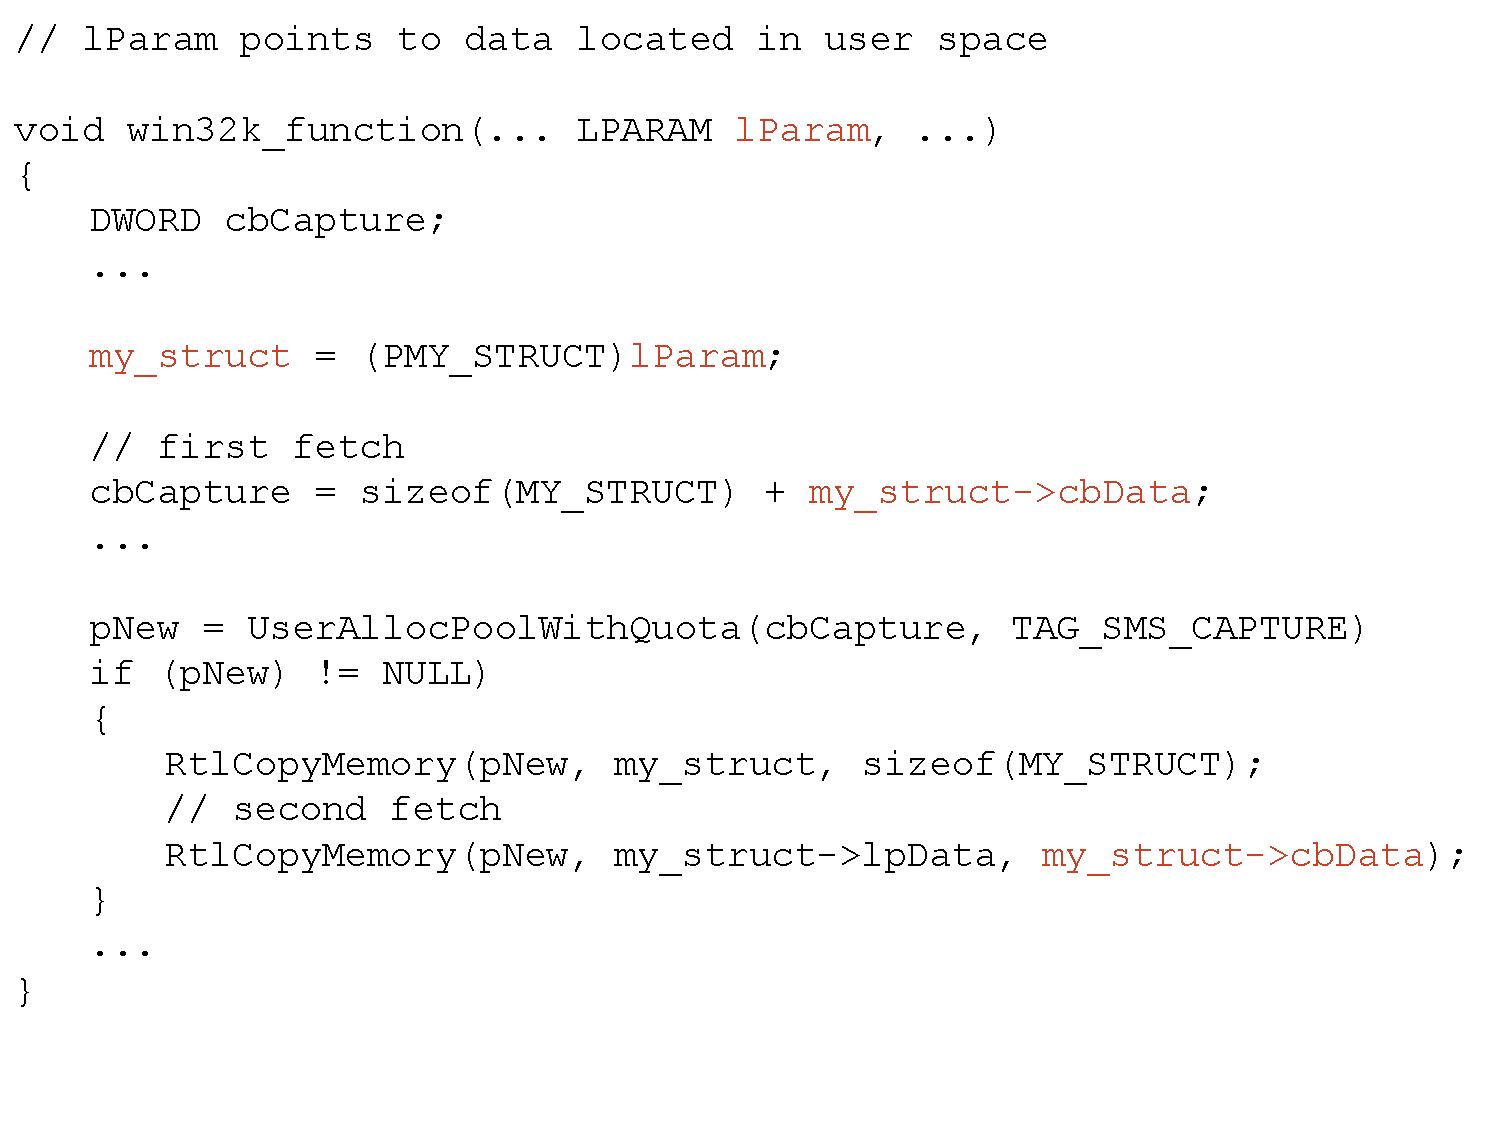
\includegraphics[width=0.47\textwidth]{toctouexample}
  \centering
  \caption{Sample code which has TOCTOU vulnerability. Data with in user space is referenced twice during a kernel pool allocation and data copying. ~\cite{jurczyk2013identifying}~\cite{ms08061}}
  \label{fig:toctouexample}
\end{figure}
\end{comment}


%lst:vulnerablecode
\begin{lstlisting}[basicstyle=\small,style=redkeyword,caption={An snippet of Windows device driver code that mimic the vulnerability that fixed in ms08-061. The vulnerable user-mode variable is marked in red.}\label{lst:vulnerablecode}]

// lParam points to data located in user space

void win32k_function(... LPARAM @lParam@, ...) 
{
    DWORD cbCapture;
    ...

    @my_struct@ = (PMY_STRUCT)@lParam@;

    // first fetch
    cbCapture = sizeof(MY_STRUCT) + @my_struct->cbData@;  
    ...

    pNew = UserAllocPoolWithQuota(cbCapture, TAG_SMS_CAPTURE)
    if (pNew != NULL) 
    {
        RtlCopyMemory(pNew, my_struct, sizeof(MY_STRUCT);
        // second fetch
        RtlCopyMemory(pNew, my_struct->lpData, @my_struct->cbData@);   
    }
    ...
}

\end{lstlisting}

Listing~\ref{lst:vulnerablecode} shows an snippet of Windows device driver code~\cite{jurczyk2013identifying} that a buffer first allocated from kernel heap, whose size is determined from a variable resides in user-mode, and later reuses that variable as a parameter in a "RtlCopyMemory" call. This is a piece of pseudo code that mimic the vulnerability that has been patched in ms08-061. "my\_struct-$>$cbData" appears two times, referencing user-mode variable, one is to determine the size of the kernel buffer (first fetch), the other is to use it as the length of data(second fetch). Since variable resides in user-mode memory could be modified by other threads, later, "my\_struct-$>$cbData" could be set to a larger value, introducing a potential kernel pool buffer overflow.

This attack can happen on both single processor system and multiple processor system. On a single processor system, even though only one thread can be scheduled to execute on the processor at a time, it's still possible to trigger the vulnerability. For example, between function calls UserAllocPoolWithQuota and RtlCopyMemory, if a thread context switch happens in between, other threads can have the opportunity to modified it.

A multiple processor environment is much more favorable to attackers. It's commonplace for both laptops or servers nowadays. Under such conditions, the attacker creates an attacking thread and use thread affinity masks to attach it to other processors. As shown in~\autoref{fig:toctouasm}. The attacking thread keeps flipping the vulnerable variable in a loop, high chance that it can successfully enlarge it during the time window. In this paper we assume the attacker captures the time window and corrupts the vulnerable value as intended. 

\begin{figure}[h]
  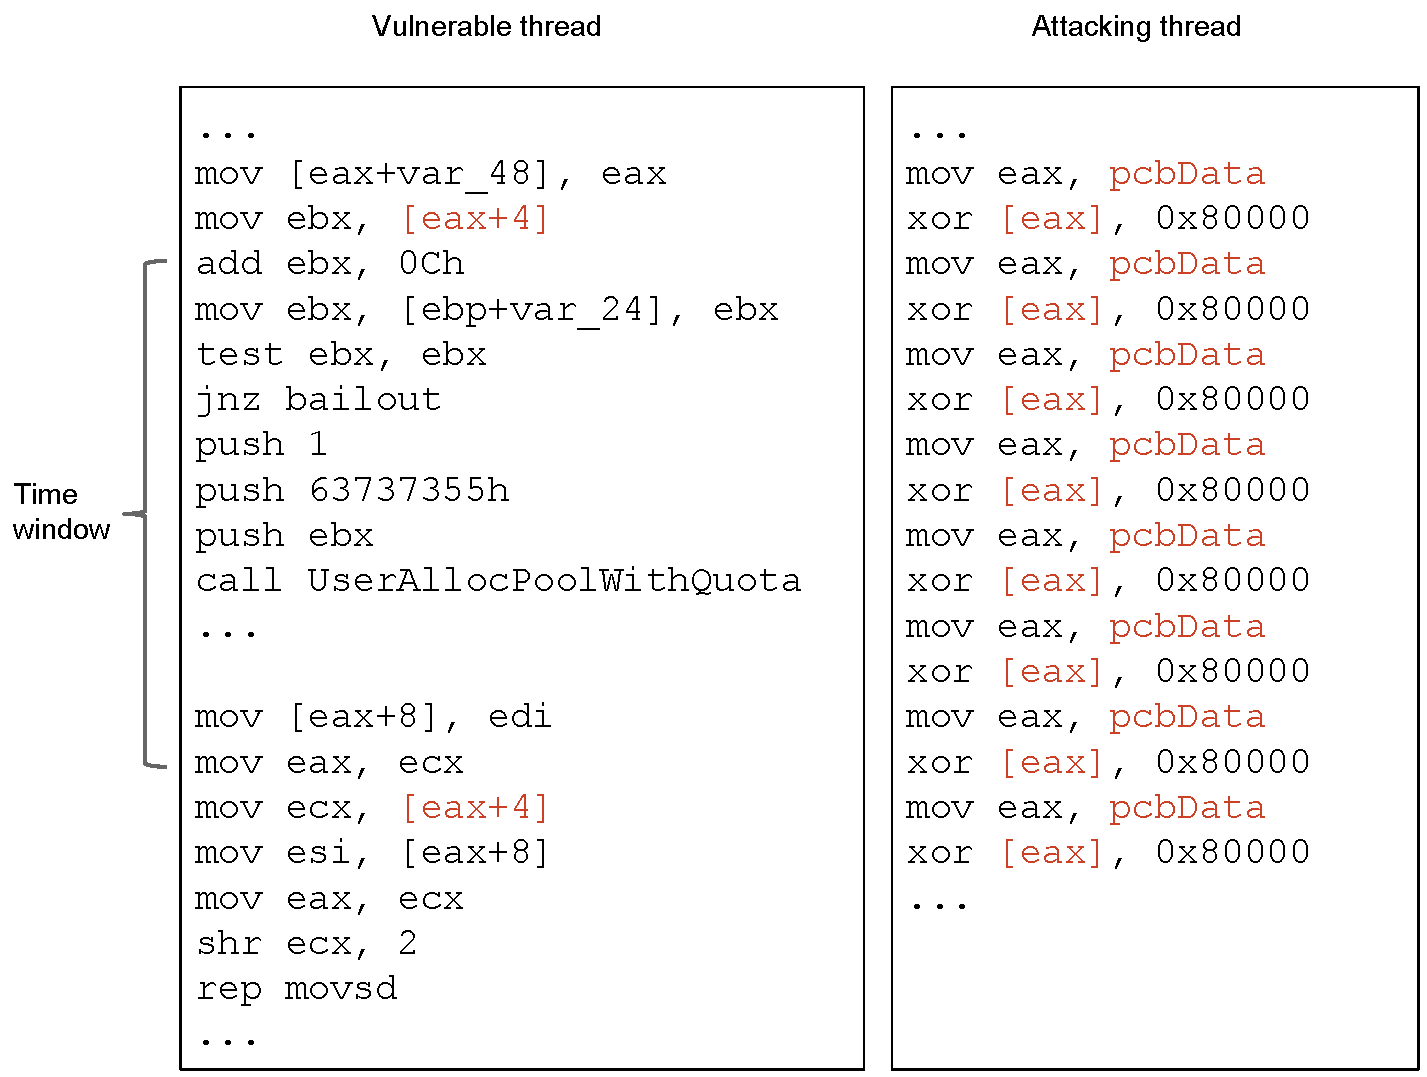
\includegraphics[width=0.47\textwidth]{figures/toctouasm}
  \centering
  \caption{The attacking thread could be as simple as several instructions in a loop.}
  \label{fig:toctouasm}
\end{figure}


\subsection{Supervisor Mode Access Prevention (SMAP)}
SMAP is a security feature of Intel processors since Broadwell microarchitecture. It prevents operating system kernel accessing user-mode memory directly, such accesses will raise an exception. This makes it harder for attackers to "trick" the kernel into using instructions or data from a user-mode program. 

Kernel code reads and writes user-mode data are commonplace. It's inevitable because user programs need to provide parameters to system calls. Therefore, two new instructions "STAC" and "CLAC" are provided to disable SMAP temporarily, giving opportunity for kernel to retrieve user data in a controllable way.

Linux kernel support for SMAP since version 3.7. All the accesses to user mode memory must go through two gateway functions copy\_to\_user() and copy\_from\_user(), where SMAP is temporarily disabled.

Windows doesn't support SMAP yet. Different from Linux's approach, each of Windows system calls tends to "probe" and "capture" user-mode data itself. Probing usually done by function ProbeForRead()~\cite{probeforread} and ProbeForWrite() to check the validity of the buffers, it also checks if a user-mode buffer actually resides in the user-mode address space by simply compare its address to a pre-defined value. Since some modules such as win32k.sys are highly coupled with user-mode components, it will cost huge engineering effort to change the way it retrieve user-mode data.

In Linux, even though copy\_*\_user() is mandated~\cite{corbet2012linuxsmap}, it still suffers from TOCTOU vulnerability such as mistake of using function copy\_from\_user() twice for the same variable~\cite{double-fetch-linux}. 
